\subsection{Feature Selection Using Decision-Tree-Classifier}

Feature selection is a crucial aspect in the preparation of modern deep learning algorithms. However, identifying the most effective method that also performs well in a live environment, such as an EVSE system with limited hardware resources, remains a challenge.\\
The paper "Enhancing EV Charging Station Security Using a Multi-dimensional Dataset" \cite{EV_Security} employed Principal Component Analysis (PCA) to reduce 900 input features for use in an LSTM model. PCA was also experimented with in this study, but due to the nature of this method, all 900 original features must still be requested in the live environment in order to compute the transformed principal components. Executing the required PromQL queries for all 900 features caused the CPU usage on the Raspberry Pi setup to average nearly 50\%, which makes this approach unsuitable for real-time deployment.\\
Following this limitation, it was necessary to explore alternative feature selection techniques that could offer high performance without requiring access to the full feature set. The paper "Comparative Analysis of Feature Selection Techniques for LSTM-Based Network Intrusion Detection Models" \cite{feature_selection} evaluated multiple feature selection strategies to determine the most effective combinations for LSTM-based algorithms.

\begin{figure}[H]
    \centering
    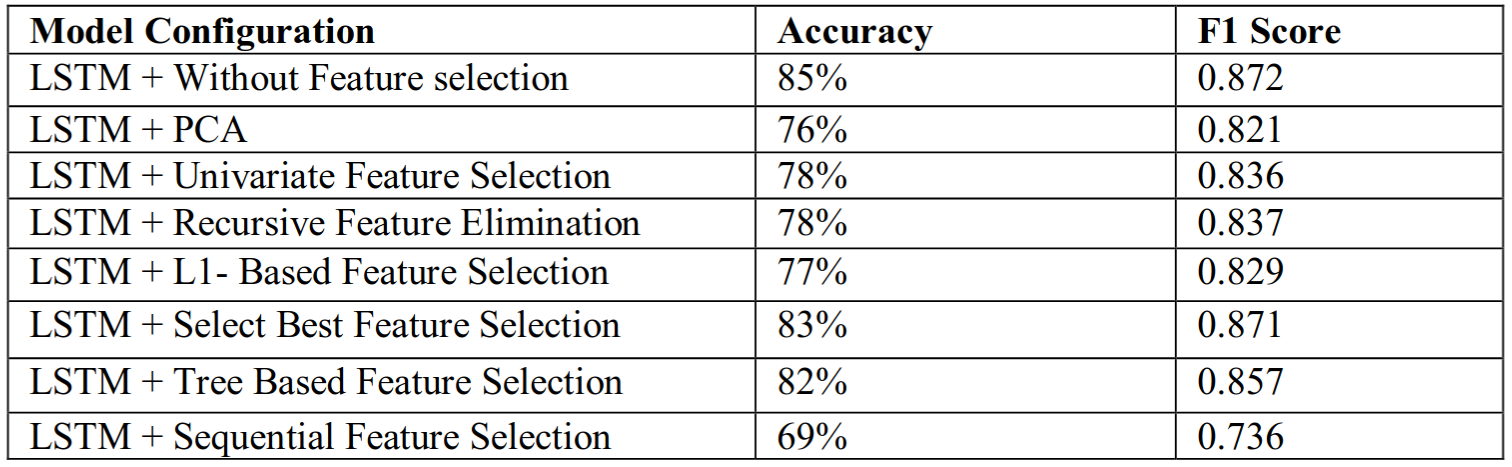
\includegraphics[width=1\textwidth]{pics/feature_selection_comparison.png}
    \caption{Comparison of feature selection methods for Long Short-Term Memory accuracy \cite{feature_selection}.}
    \label{fig:feature_selection_comparison}
\end{figure}
According to their findings, the LSTM model without any feature selection achieved the highest accuracy at 85\%. However, as previously mentioned, using all 900 features is not feasible in the hardware-constrained environment. The next best accuracies were achieved using LSTM combined with either the "Select Best Feature Selection method" or "Tree-Based feature selection," with only a 1\% accuracy drop and an F1-score difference of just 0.014.\\
Given this background, the Decision Tree algorithm was adopted for feature selection. This allows identification of the most relevant features while maintaining a high level of accuracy and keeping resource usage within system constraints.\\

% Explanation of the Decision Tree setup for feature selection
With this information, a Decision Tree was created to select the most relevant features for real-time detection in the EVSE system. The Decision-Tree-Classifier from the \texttt{sklearn.tree} module was used, as it is easy to use and integrates well with common data science workflows.\\

In this step, the preprocessed dataset was used to train a Decision-Tree-Classifier for feature selection. First, the categorical labels were converted into a binary format, where benign was mapped to 0 and attack to 1. To prevent data leakage, the columns label, timestamp, and attack were dropped from the feature set before training. The Decision-Tree-Classifier was then trained on the remaining features using a fixed random seed (\texttt{random\_state=42}). This model primarily served to identify the most relevant features for subsequent analysis and classification tasks.\\
This approach allowed significant reduction of the number of input features while preserving high detection accuracy and runtime performance.


% Visualizations for feature selection (Confusion Matrix, Correlation Matrix, Feature Importance)
\begin{figure}[H]
    \centering
    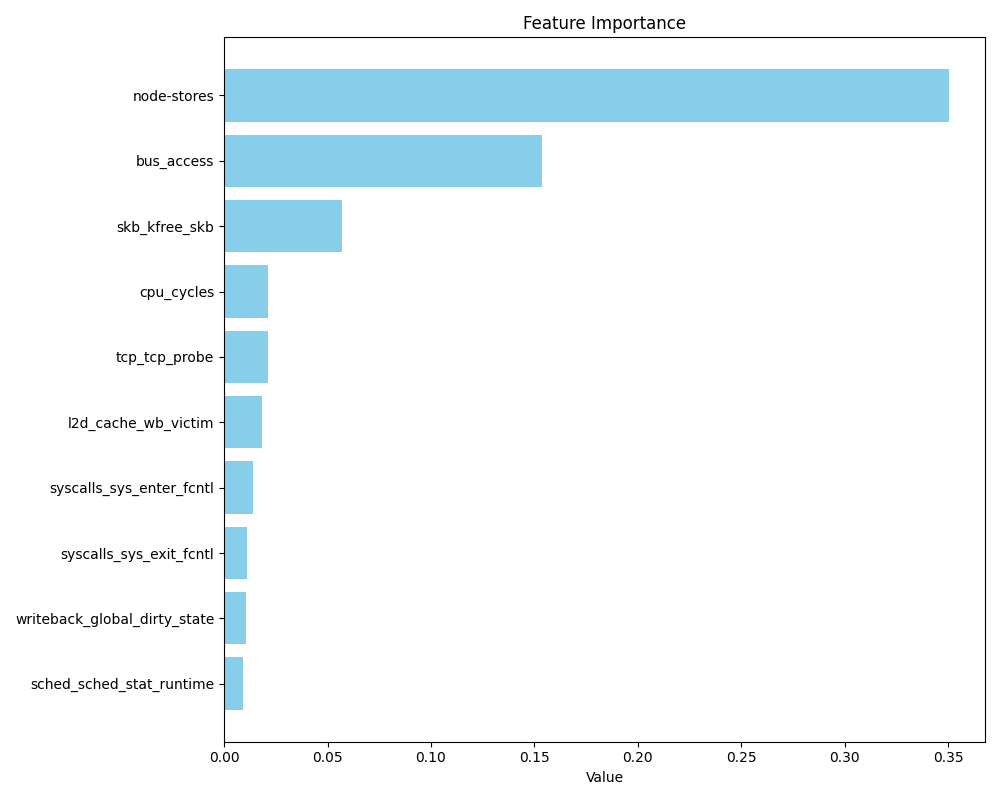
\includegraphics[width=0.8\textwidth]{pics/feature_importance.png}
    \caption{Top 10 most important features selected by the Decision-Tree-Classifier.}
    \label{fig:feature_importance}
\end{figure}

\paragraph{\texttt{node-stores}:} This event refers to memory store operations targeting specific NUMA nodes in a multi-node system. Monitoring \texttt{node-stores} events help analyze memory access patterns and data locality \cite{nodestore_explained}, which can be important to detect unusual memory write activity often seen during attacks like UDP-Flood or ICMP-Flood where large volumes of data are rapidly written.

\paragraph{\texttt{bus-access}:} This event tracks accesses on the system bus, responsible for communication between CPUs, memory, and peripheral devices \cite{busaccess_explained}. Elevated or abnormal \texttt{bus-access} patterns can indicate intensive network or port scanning activities such as Portscans or Aggressive-Scan that generate many small requests to different system resources.

\paragraph{\texttt{skb\_kfree\_skb}:} This tracepoint event in the Linux kernel occurs when socket buffers (SKBs) managing network packets are freed \cite{skbkfree_explained}. Tracking this event is crucial for detecting attacks that flood or manipulate network connections, including Slowloris (many half-open connections), SYN-Flood (half-open TCP connections), UDP-Flood, and ICMP-Flood, because these attacks cause unusually high packet processing and freeing activity.\\

Using the 20 most important features identified by the Decision-Tree-Classifier, a correlation matrix was created to examine feature redundancy.

\begin{figure}[H]
    \centering
    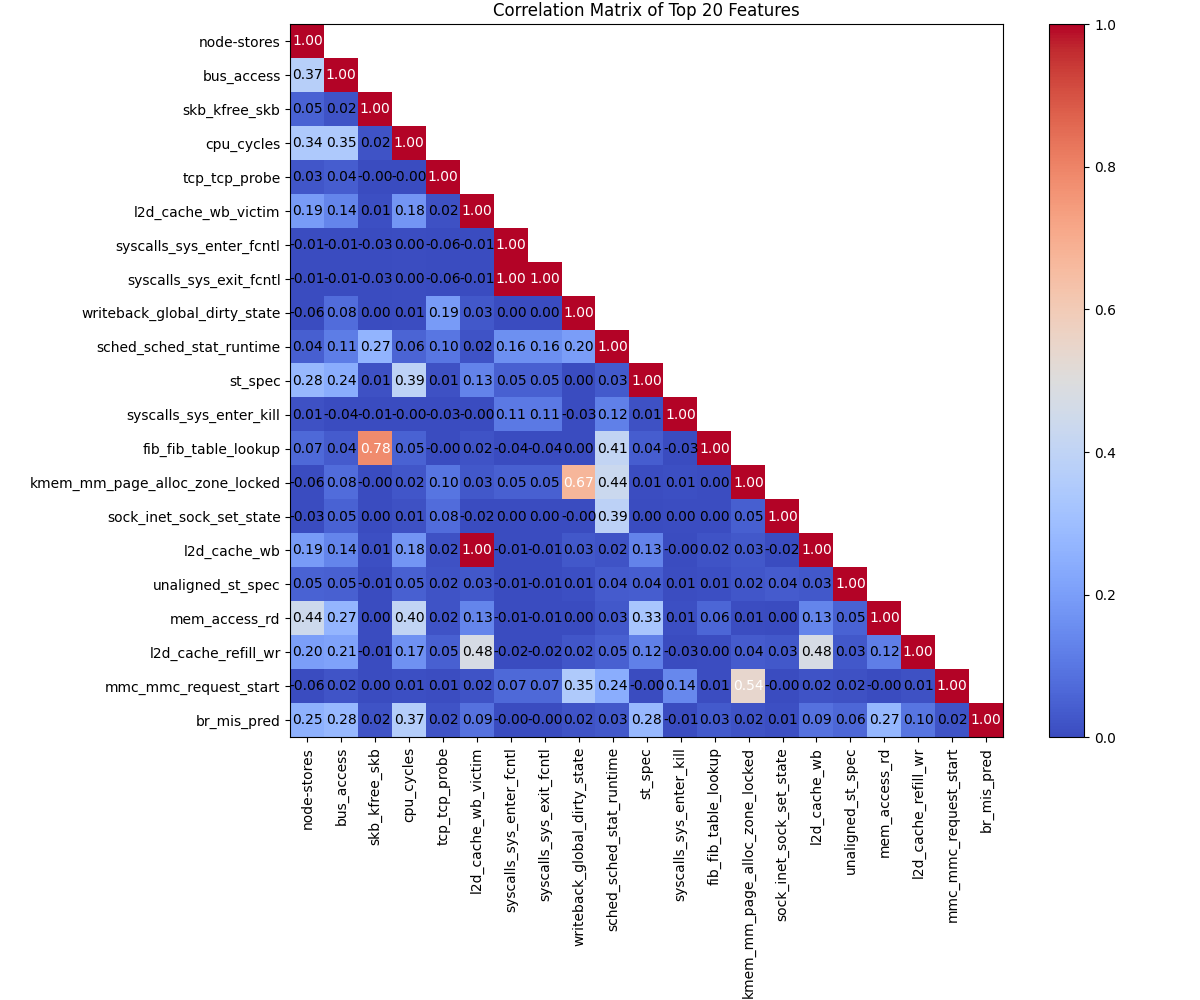
\includegraphics[width=1\textwidth]{pics/corrlationMatrix_DT.png}
    \caption{Correlation matrix top Features with Decision-Tree-Classifier.}
    \label{fig:corrlationMatrix_DT}
\end{figure}

The correlation matrix in Figure~\ref{fig:corrlationMatrix_DT} shows that there is almost no correlation between the top 20 features selected by the Decision-Tree-Classifier. This result is highly desirable, as it indicates that the chosen features are largely independent from one another and therefore provide complementary information rather than redundant signals. In practice, this means that the model can learn from a broad spectrum of system behaviors instead of being biased toward multiple highly correlated indicators of the same phenomenon. \\

For the LSTM-based detection model later, this independence between features is particularly beneficial. LSTMs are designed to capture temporal dependencies and patterns in sequential data, and providing them with a diverse set of non-redundant input signals increases their ability to generalize across different attack types and benign conditions \cite{lstm_feature_selection}. Furthermore, reducing feature correlation improves computational efficiency, as the system does not waste resources processing multiple overlapping signals. Overall, the low correlation among the selected features represents an optimal foundation for training the LSTM model in a resource-constrained environment.\\

Applying the same Decision-Tree-Classifier to the CICEVSE2024 dataset naturally produces different results, as the features exhibit different peaks and benign data patterns, which were already observed earlier. 
\begin{figure}[h]
    \centering
    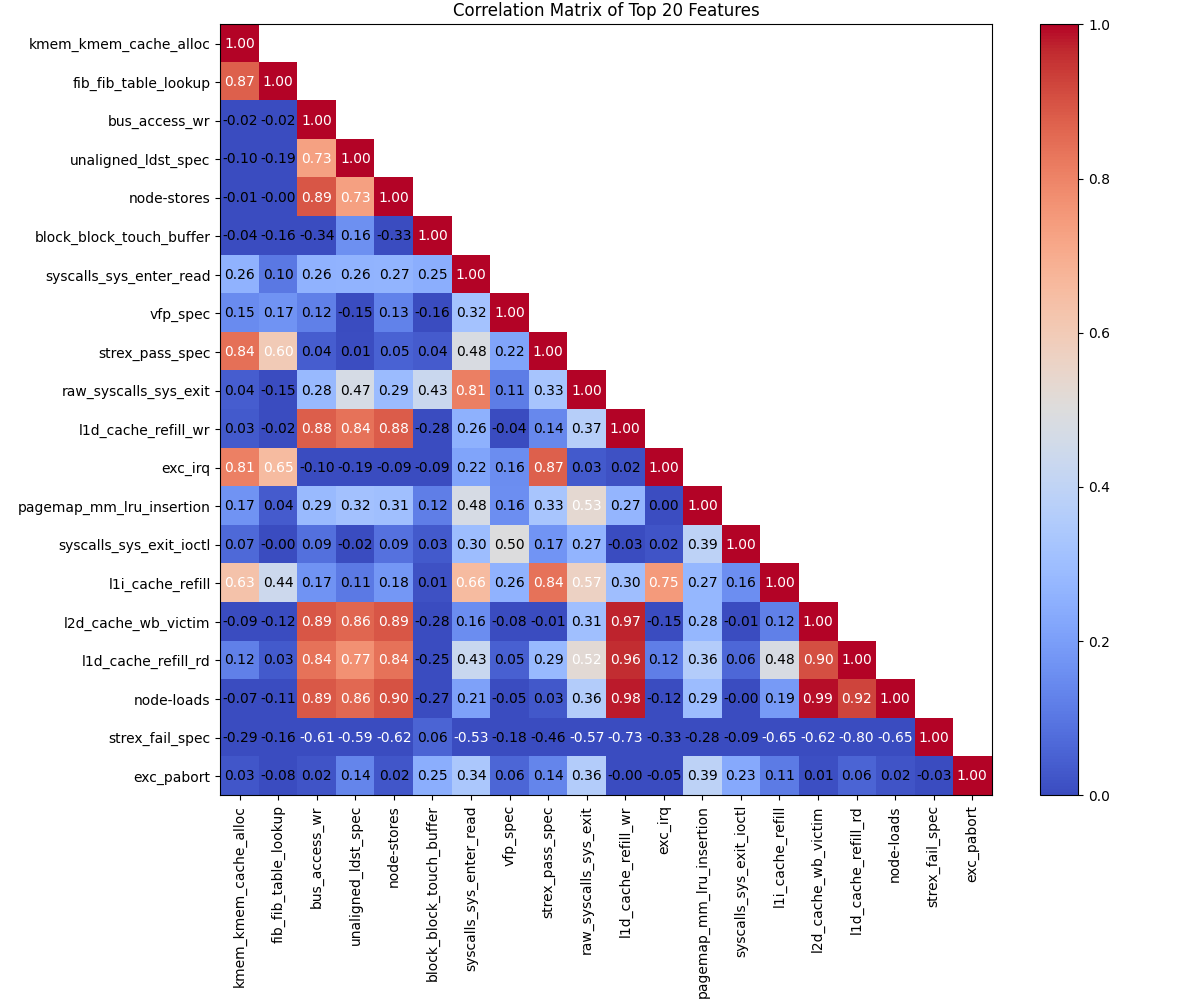
\includegraphics[width=1\textwidth]{pics/corrlationMatrix_DT_public.png}
    \caption{Correlation matrix of top features selected by the Decision-Tree-Classifier on the CICEVSE2024 dataset.}
    \label{fig:corrlationMatrix_DT_public}
\end{figure}

Nevertheless, some correlations among the selected features can still be observed. For example, in both datasets, features such as \texttt{node-stores}, \texttt{l2d\_cache\_wb\_victim}, and \texttt{fib\_fib\_table\_lookup} were consistently selected. The \texttt{l2d\_cache\_wb\_victim} event represents write-back operations of the Level 2 data cache for evicted “victim” lines, indicating high memory traffic due to cache evictions under intensive load conditions, such as flooding attacks. The \texttt{fib\_fib\_table\_lookup} event is triggered during routing table lookups in the kernel’s forwarding information base, reflecting increased network routing activity common in scanning or flood attacks. Similarly, the \texttt{skb\_kfree\_skb} and \texttt{fib\_fib\_table\_lookup} features also show a strong correlation, which is particularly evident in Figure \ref{fig:skb_fib_timeline}. The \texttt{skb\_kfree\_skb} event occurs when socket buffers managing network packets are freed, a critical indicator of network connection flooding or manipulation seen in attacks such as Slowloris, SYN-Floods, UDP-Flood, and ICMP-Floods. These interrelations highlight complementary aspects of network and memory behavior under attack scenarios.

\begin{figure}[H]
    \centering
    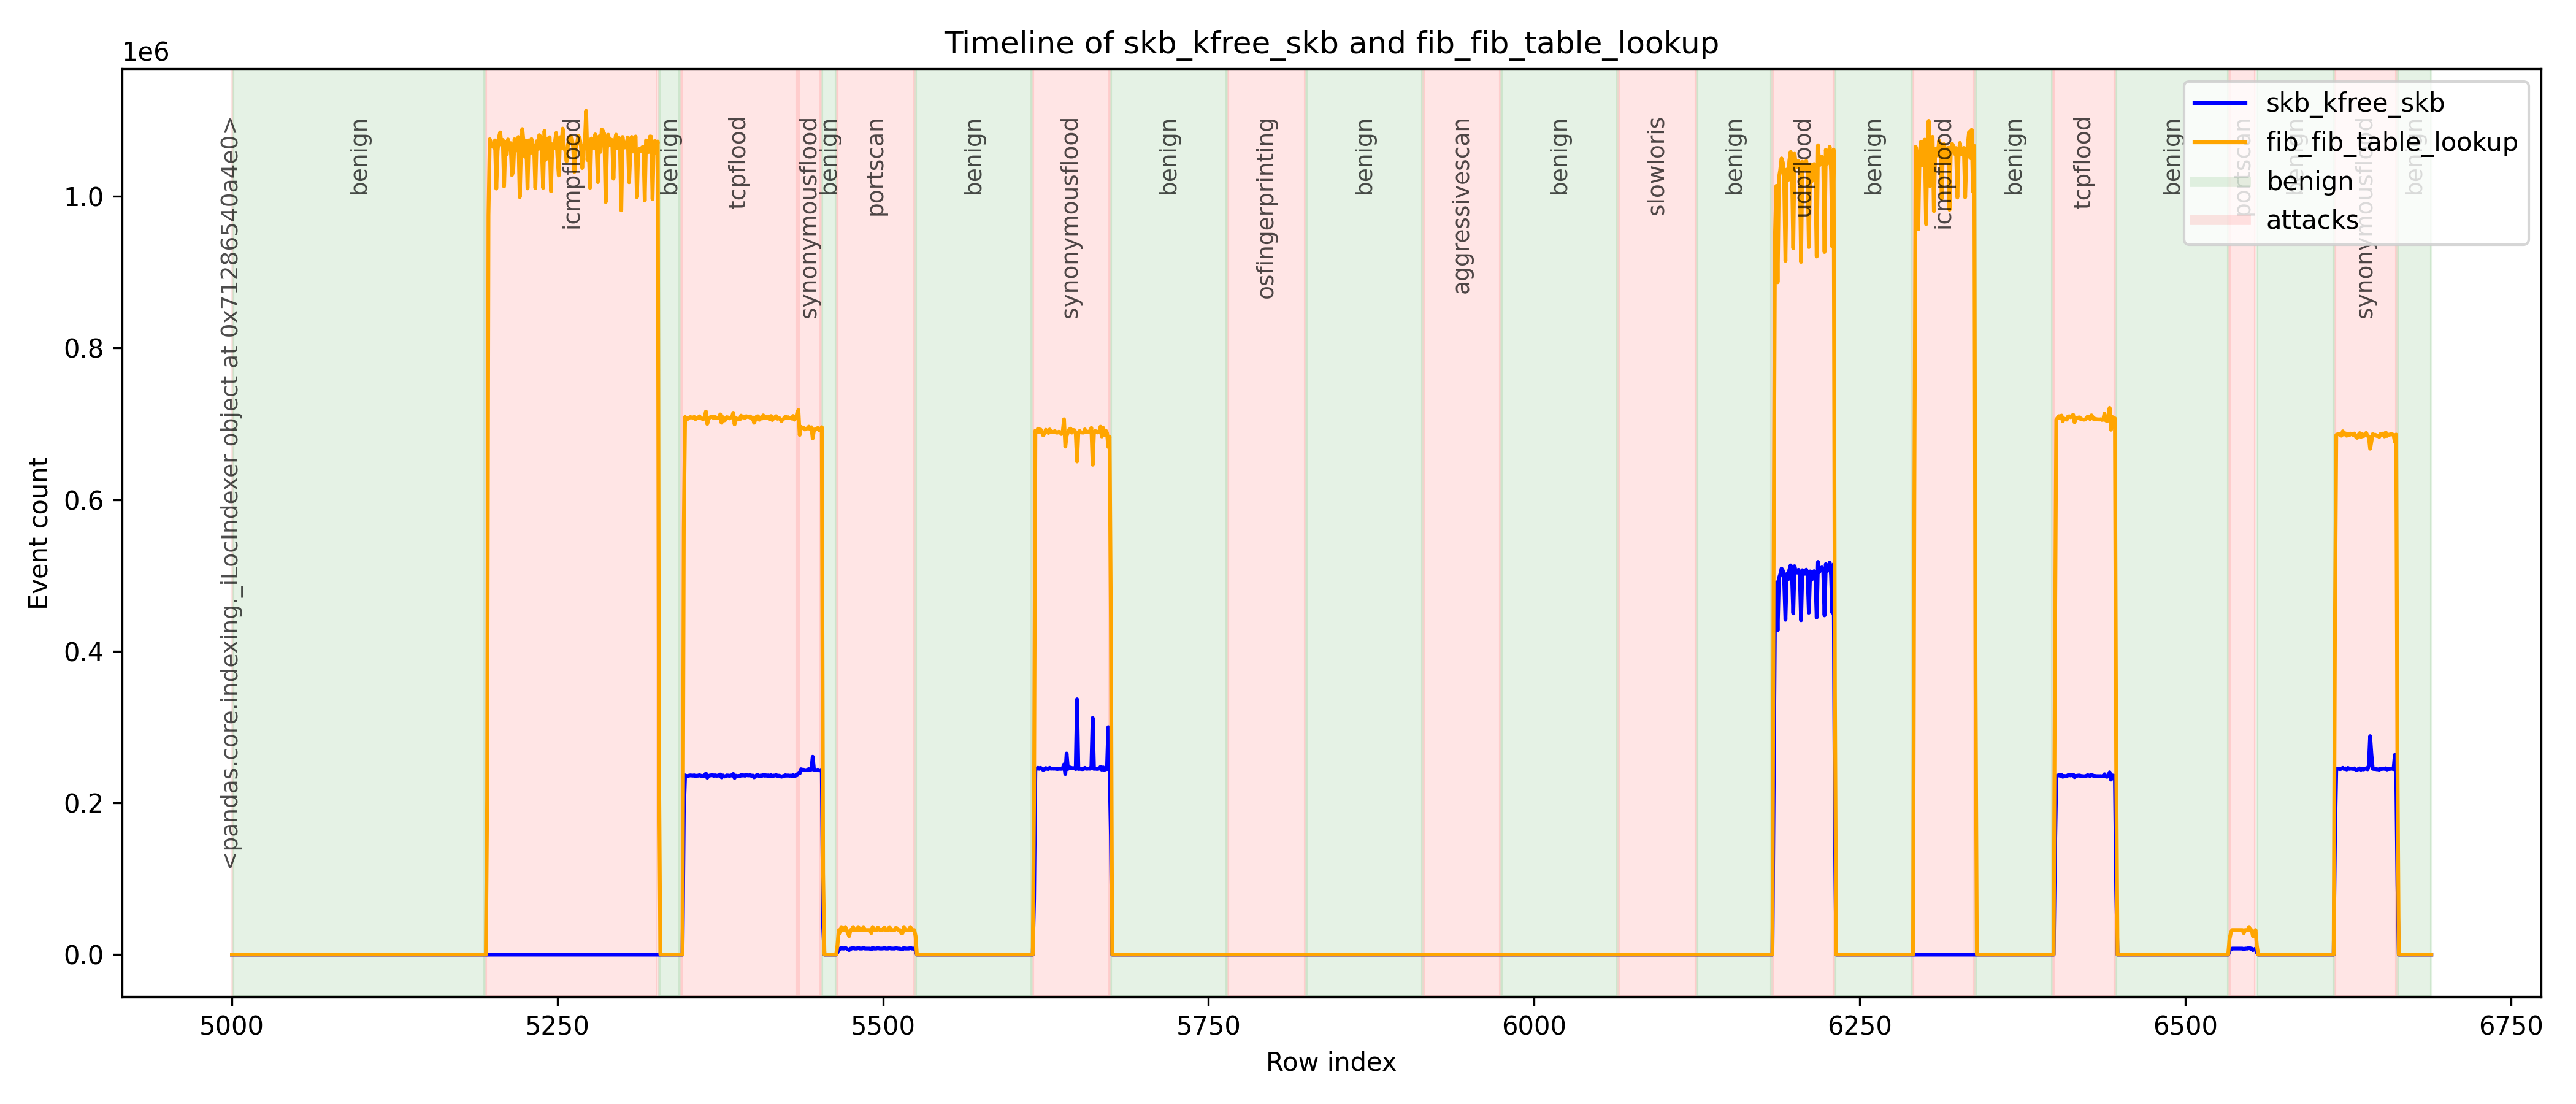
\includegraphics[width=1\textwidth]{pics/skb_fib_timeline.png}
    \caption{Correlation between \texttt{skb\_kfree\_skb} and \texttt{fib\_fib\_table\_lookup} features.}
    \label{fig:skb_fib_timeline}
\end{figure}

So far, it has been observed that the Decision-Tree-Classifier selects similar features in both datasets. This indicates that it is likely to select comparable features in other, similarly structured setups, even when more than 900 potential features are available. However, the strongest predictive power is concentrated in only a small subset of these features.\\

It is essential to examine the selected features in the context of the timeline in order to better understand their behavior and patterns over time and to assess whether they are useful for the LSTM algorithm in detecting attacks. In this work, a detailed discussion of every individual feature is not provided; instead, all corresponding figures can be found in the appendix.\\

As already observed, the \texttt{node-stores} feature shows a clear pattern that helps in detecting flooding attacks, as described before, while the \texttt{sys\_calls\_sys\_enter\_kill} feature records the number of times the Linux kernel processes the ``kill'' system call (i.e., \texttt{sys\_kill}), which is used by processes to send signals to other processes. During a Portscan attack, tools such as \texttt{nmap} or similar scanners attempt to rapidly open and close many connections across a wide range of ports. This aggressive probing leads to the frequent creation and termination of network sockets and, in some cases, the spawning of short-lived processes for each connection attempt.\\
In summary, the high peaks in \texttt{sys\_calls\_sys\_enter\_kill} during Portscan attacks reflect the system's intensive signaling behavior as it deals with the rapid creation and destruction of connections and processes, making it a strong indicator for detecting such attacks.

\begin{figure}[H]
    \centering
    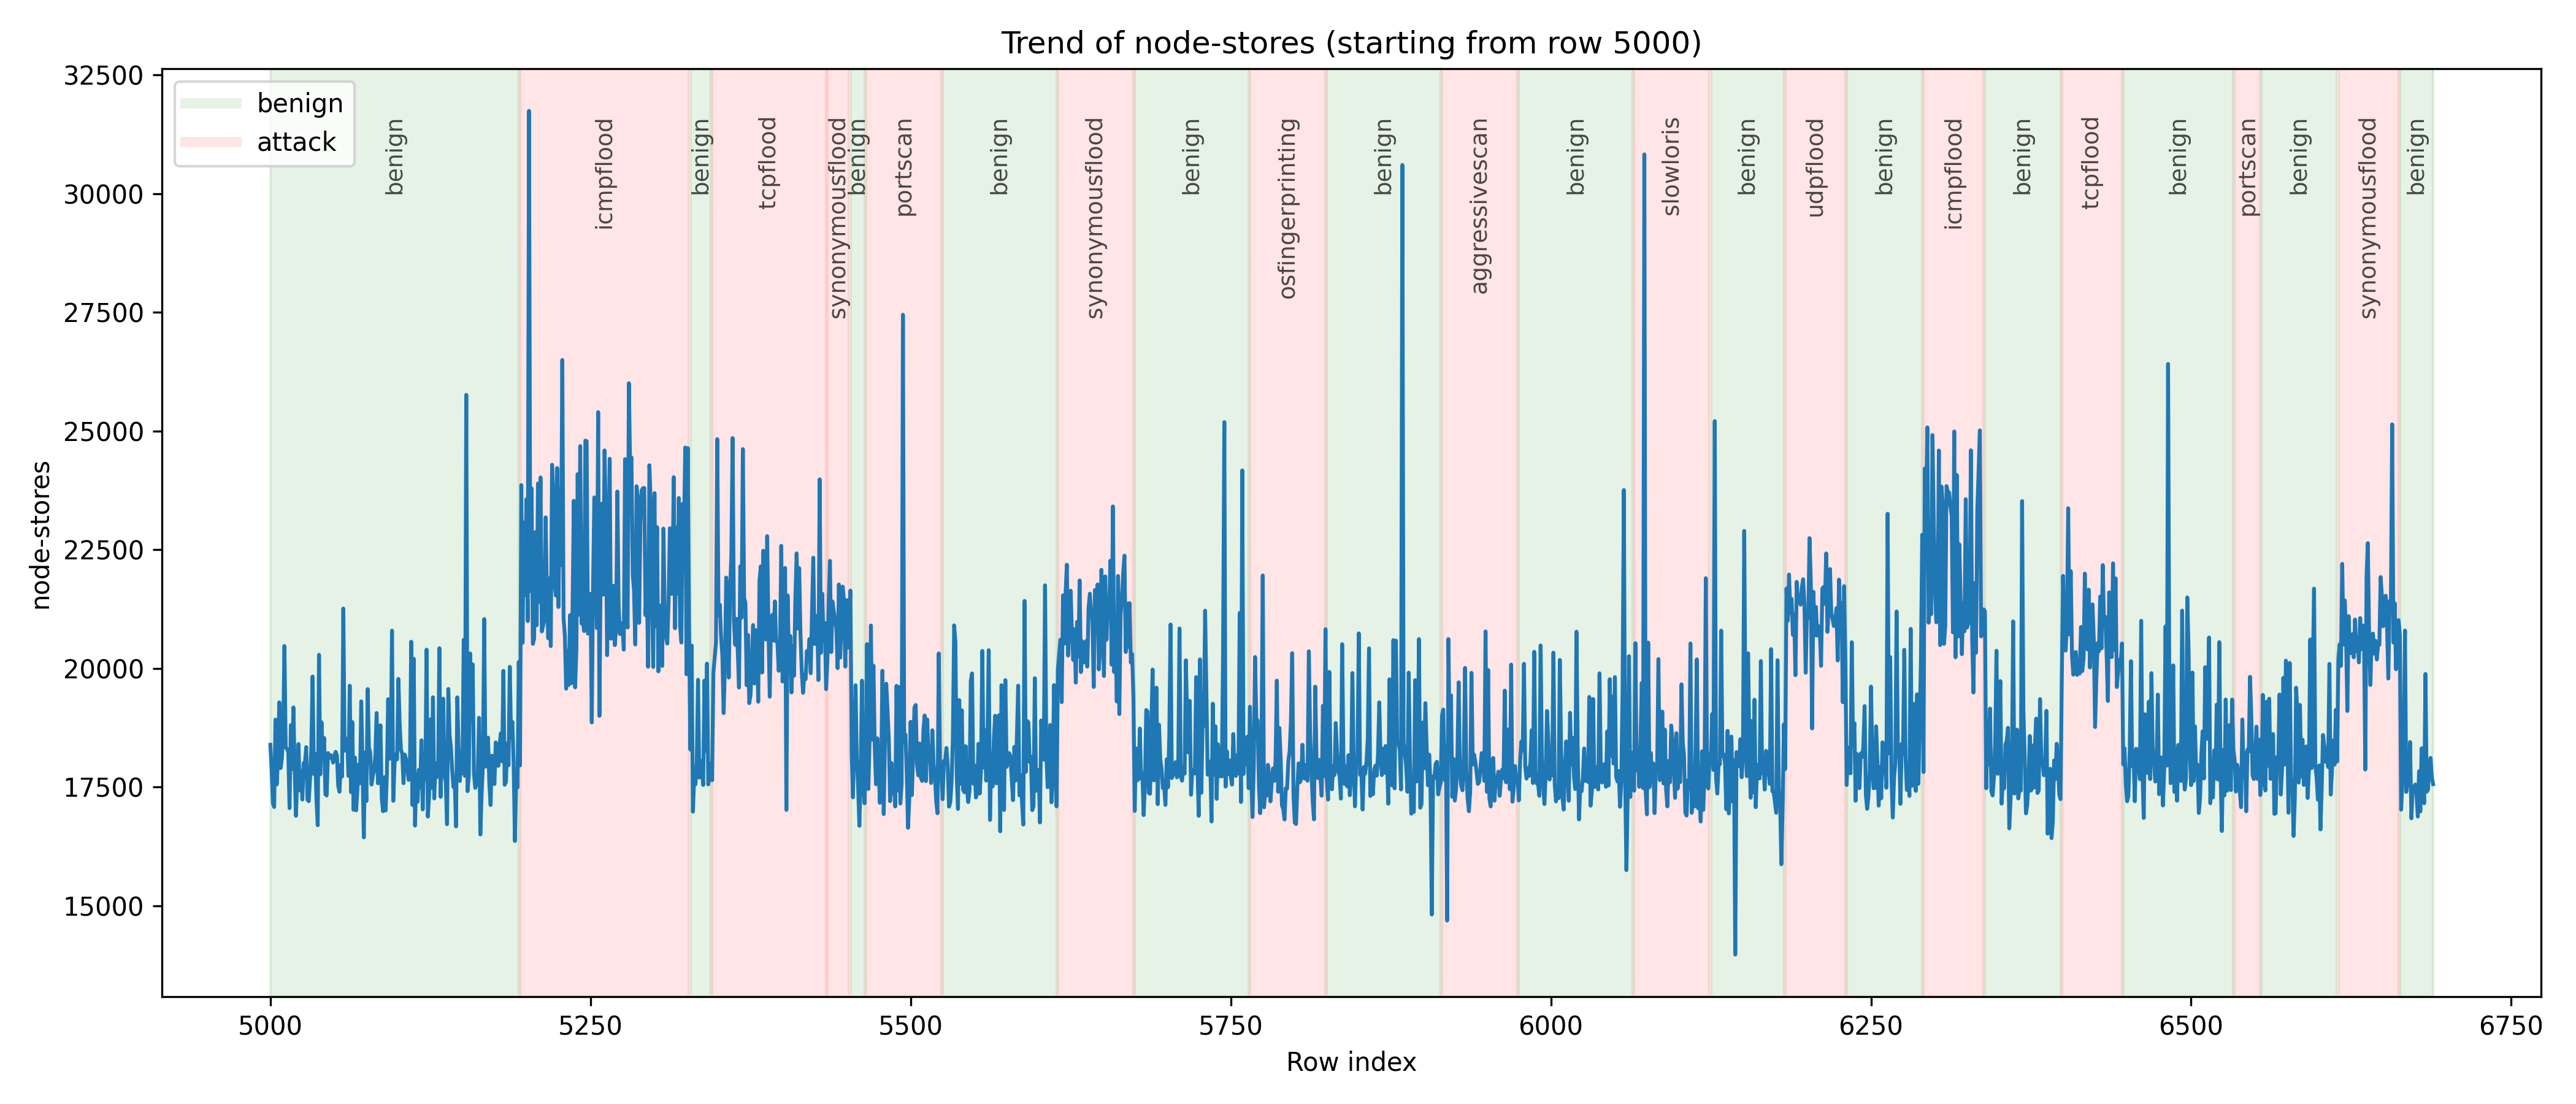
\includegraphics[width=0.9\textwidth]{pics/node-stores.png}
    \caption{Timeline behavior of the \texttt{node-stores} feature, showing distinguishable patterns during flooding attacks.}
    \label{fig:node_stores_timeline}
\end{figure}
\begin{figure}[H]
    \centering
    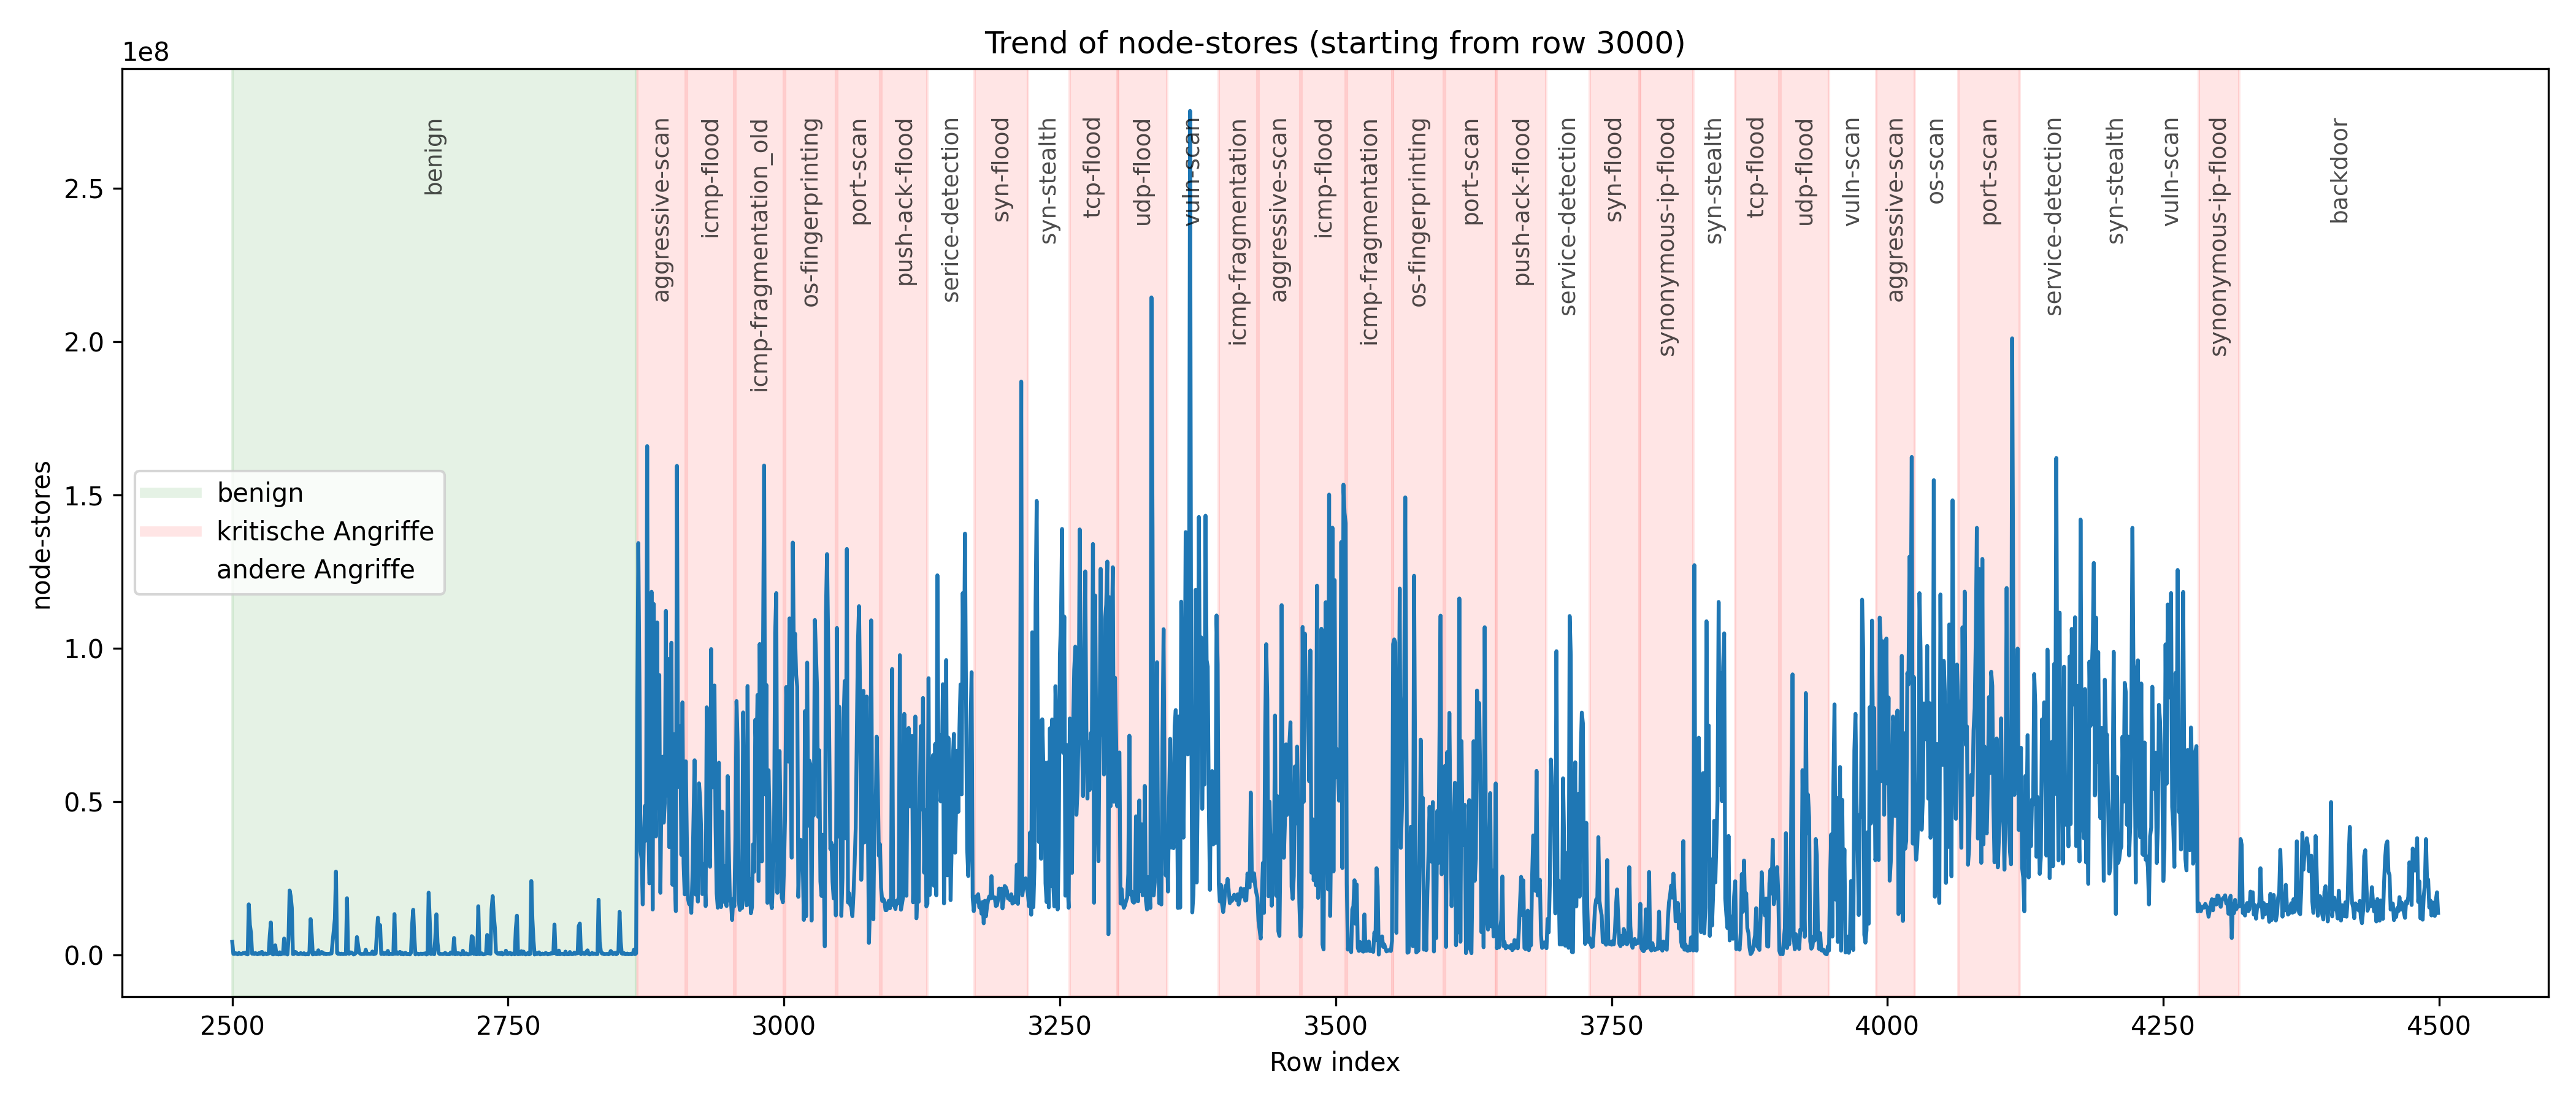
\includegraphics[width=0.9\textwidth]{pics/node-stores_public.png}
    \caption{Timeline behavior of the \texttt{node-stores} feature from the CICEVSE2024 dataset.}
    \label{fig:stores_public_timeline}
\end{figure}

\begin{figure}[H]
    \centering
    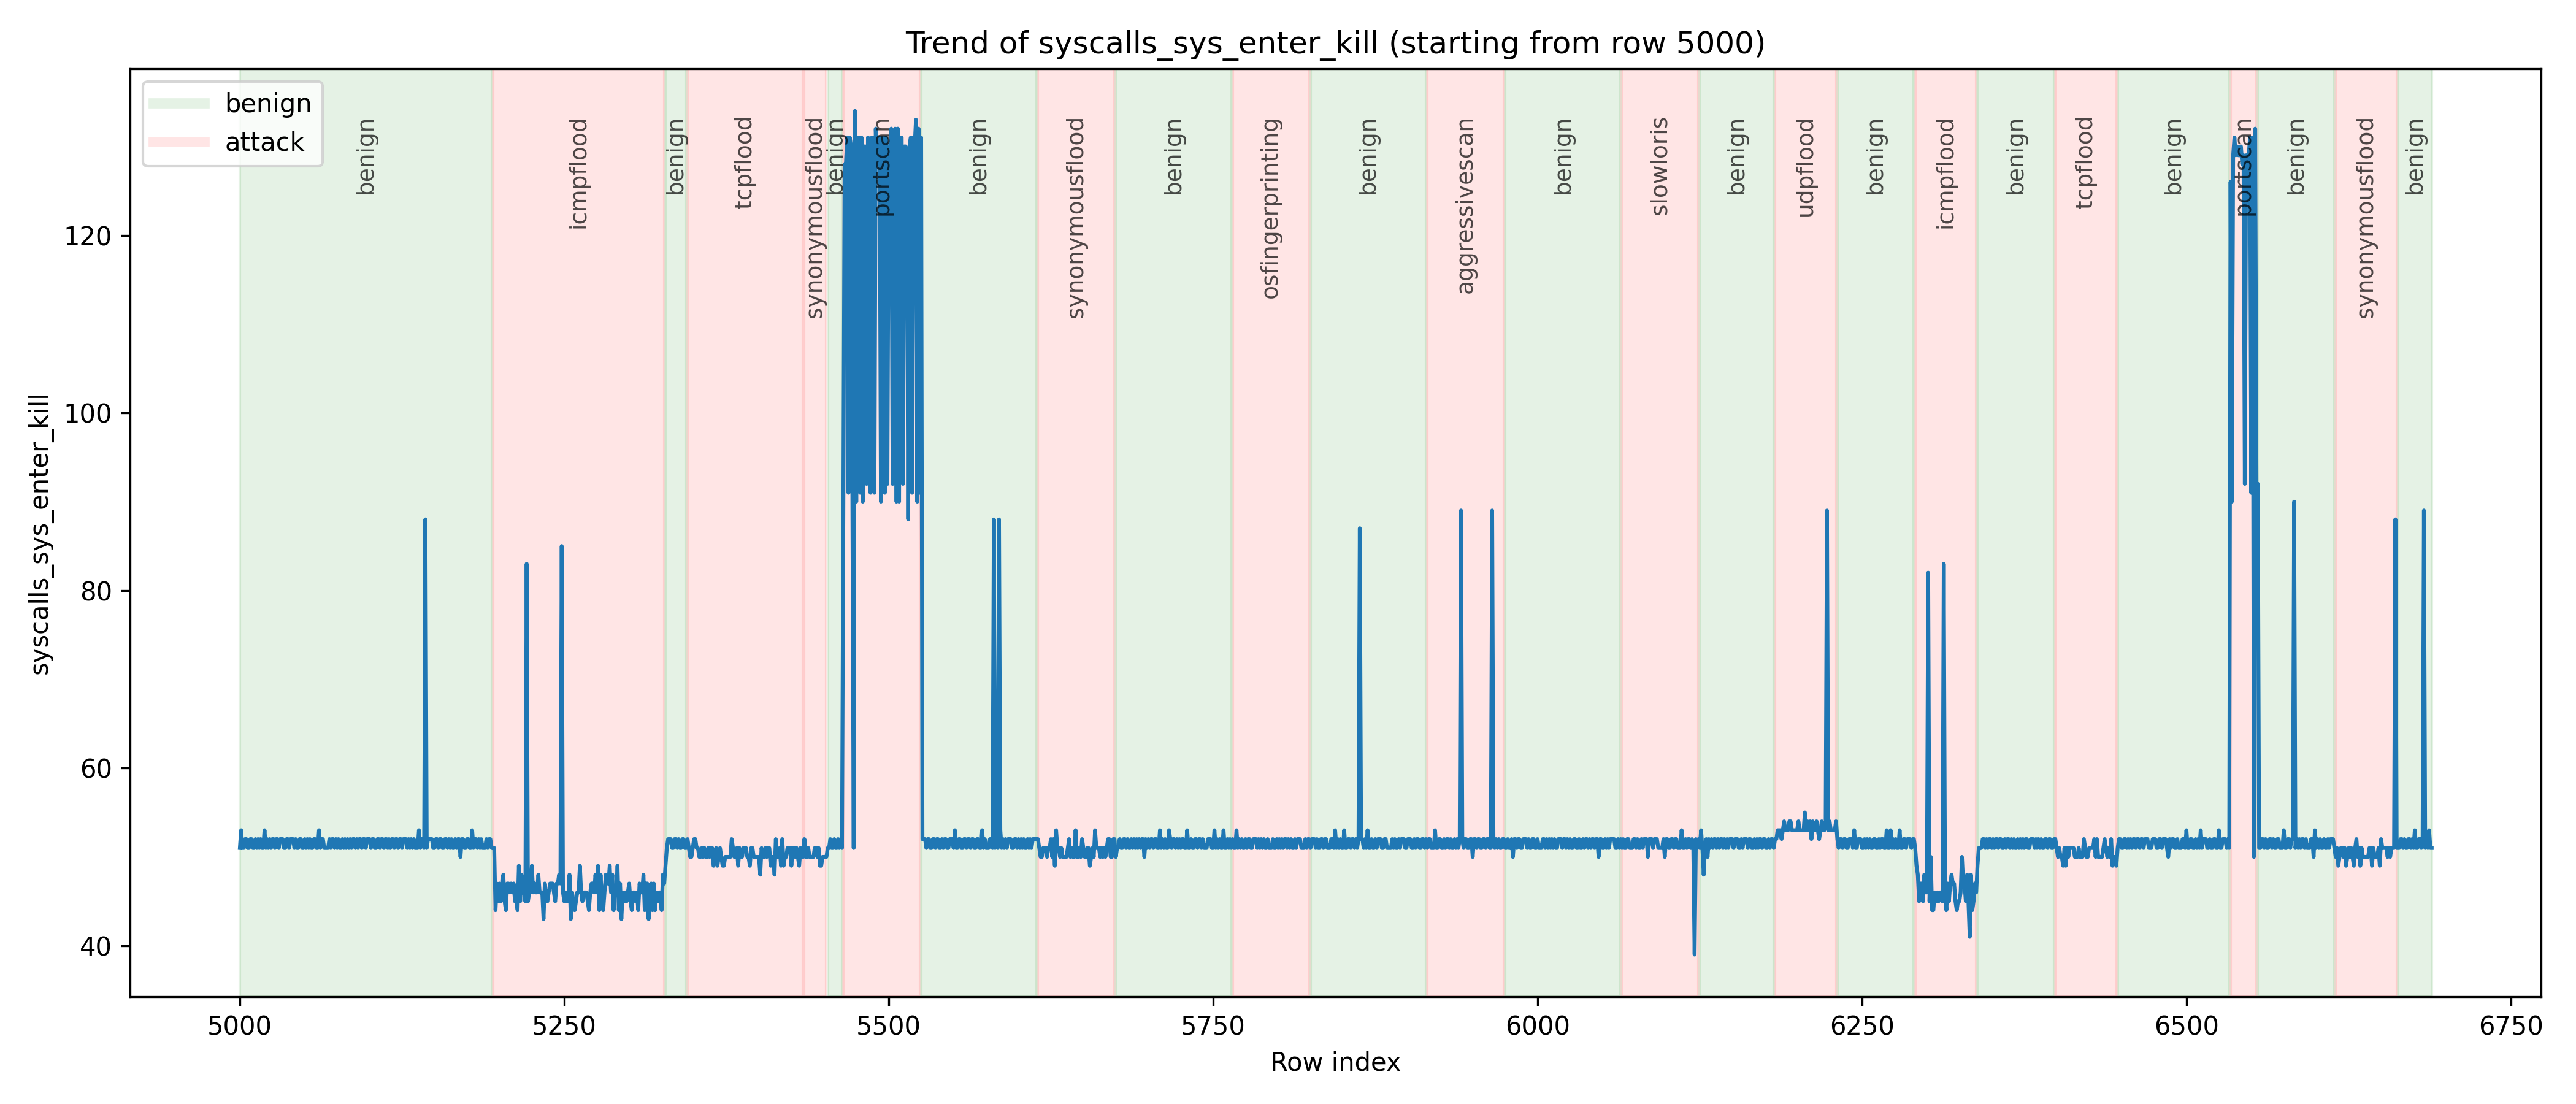
\includegraphics[width=0.9\textwidth]{pics/syscalls_sys_enter_kill.png}
    \caption{Timeline behavior of the \texttt{sys\_calls\_sys\_enter\_kill} feature, highlighting its usefulness in detecting Portscan attacks.}
    \label{fig:sys_enter_kill_timeline}
\end{figure}
\begin{figure}[H]
    \centering
    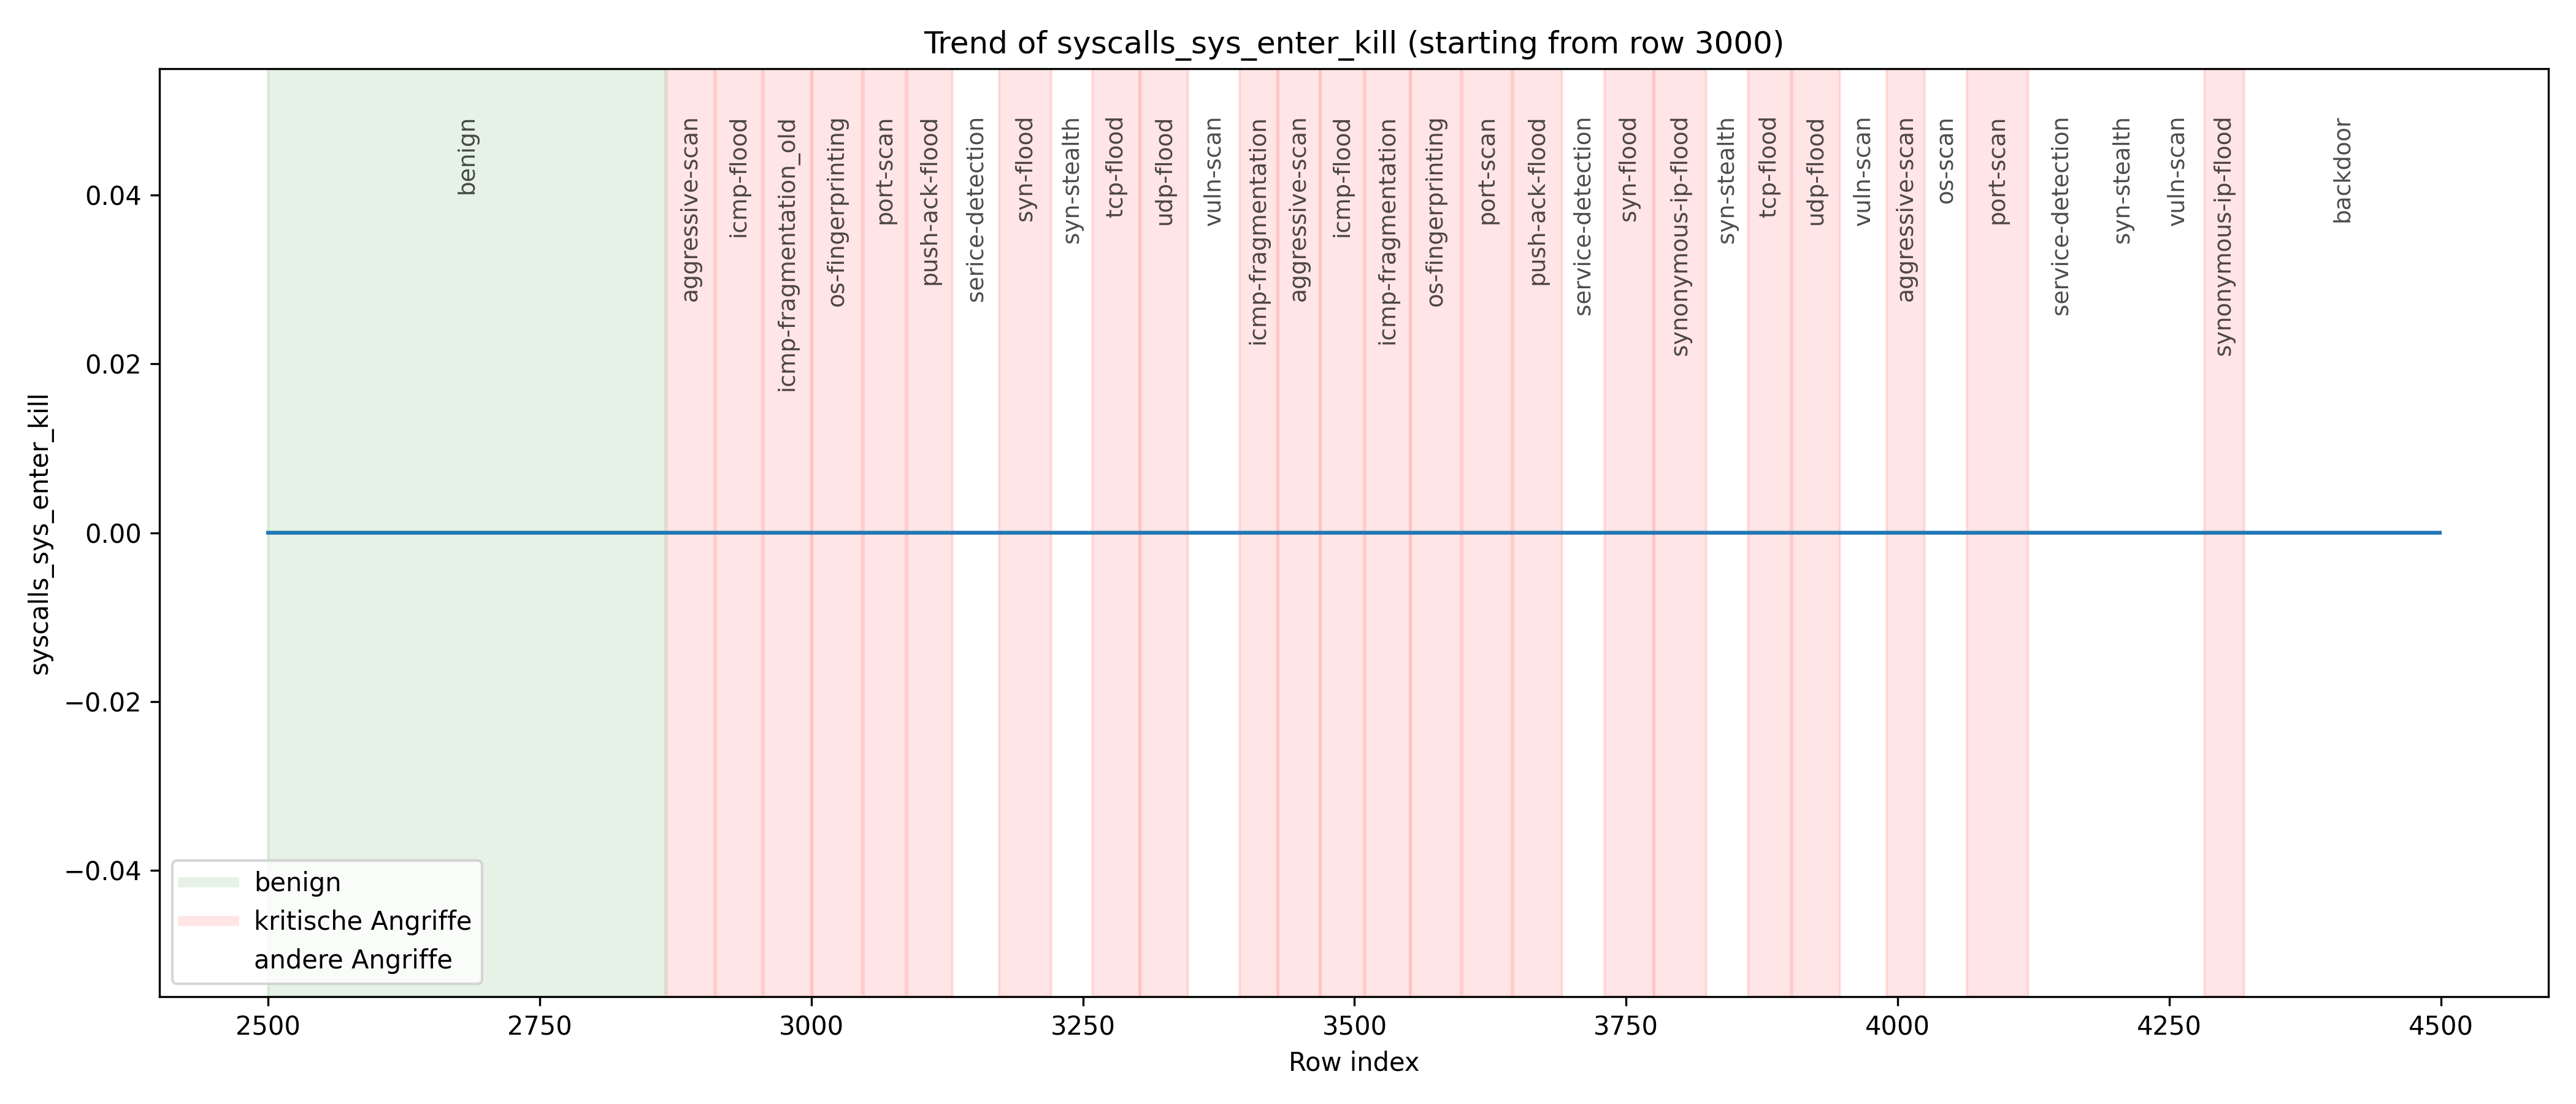
\includegraphics[width=0.9\textwidth]{pics/syscalls_sys_enter_kill_public.png}
    \caption{Timeline behavior of the \texttt{sys\_calls\_sys\_enter\_kill} feature, from the CICEVSE2024 dataset. The lack of variation in the feature within the CICEVSE2024 dataset may be due to a measurement error or the system call not being invoked during the entire monitoring period. Unfortunately, neither the paper \cite{EV_Security} nor the accompanying dataset provides a definitive explanation.}
    \label{fig:syscalls_sys_enter_kill_public_timeline}
\end{figure}

On the other hand, some features are unfortunately not very useful for attack detection, as they show almost no distinguishable peaks between benign and attack data. This is the case for the feature \texttt{unaligned\_st\_spec}, as illustrated in the figure below.  

\begin{figure}[H]
    \centering
    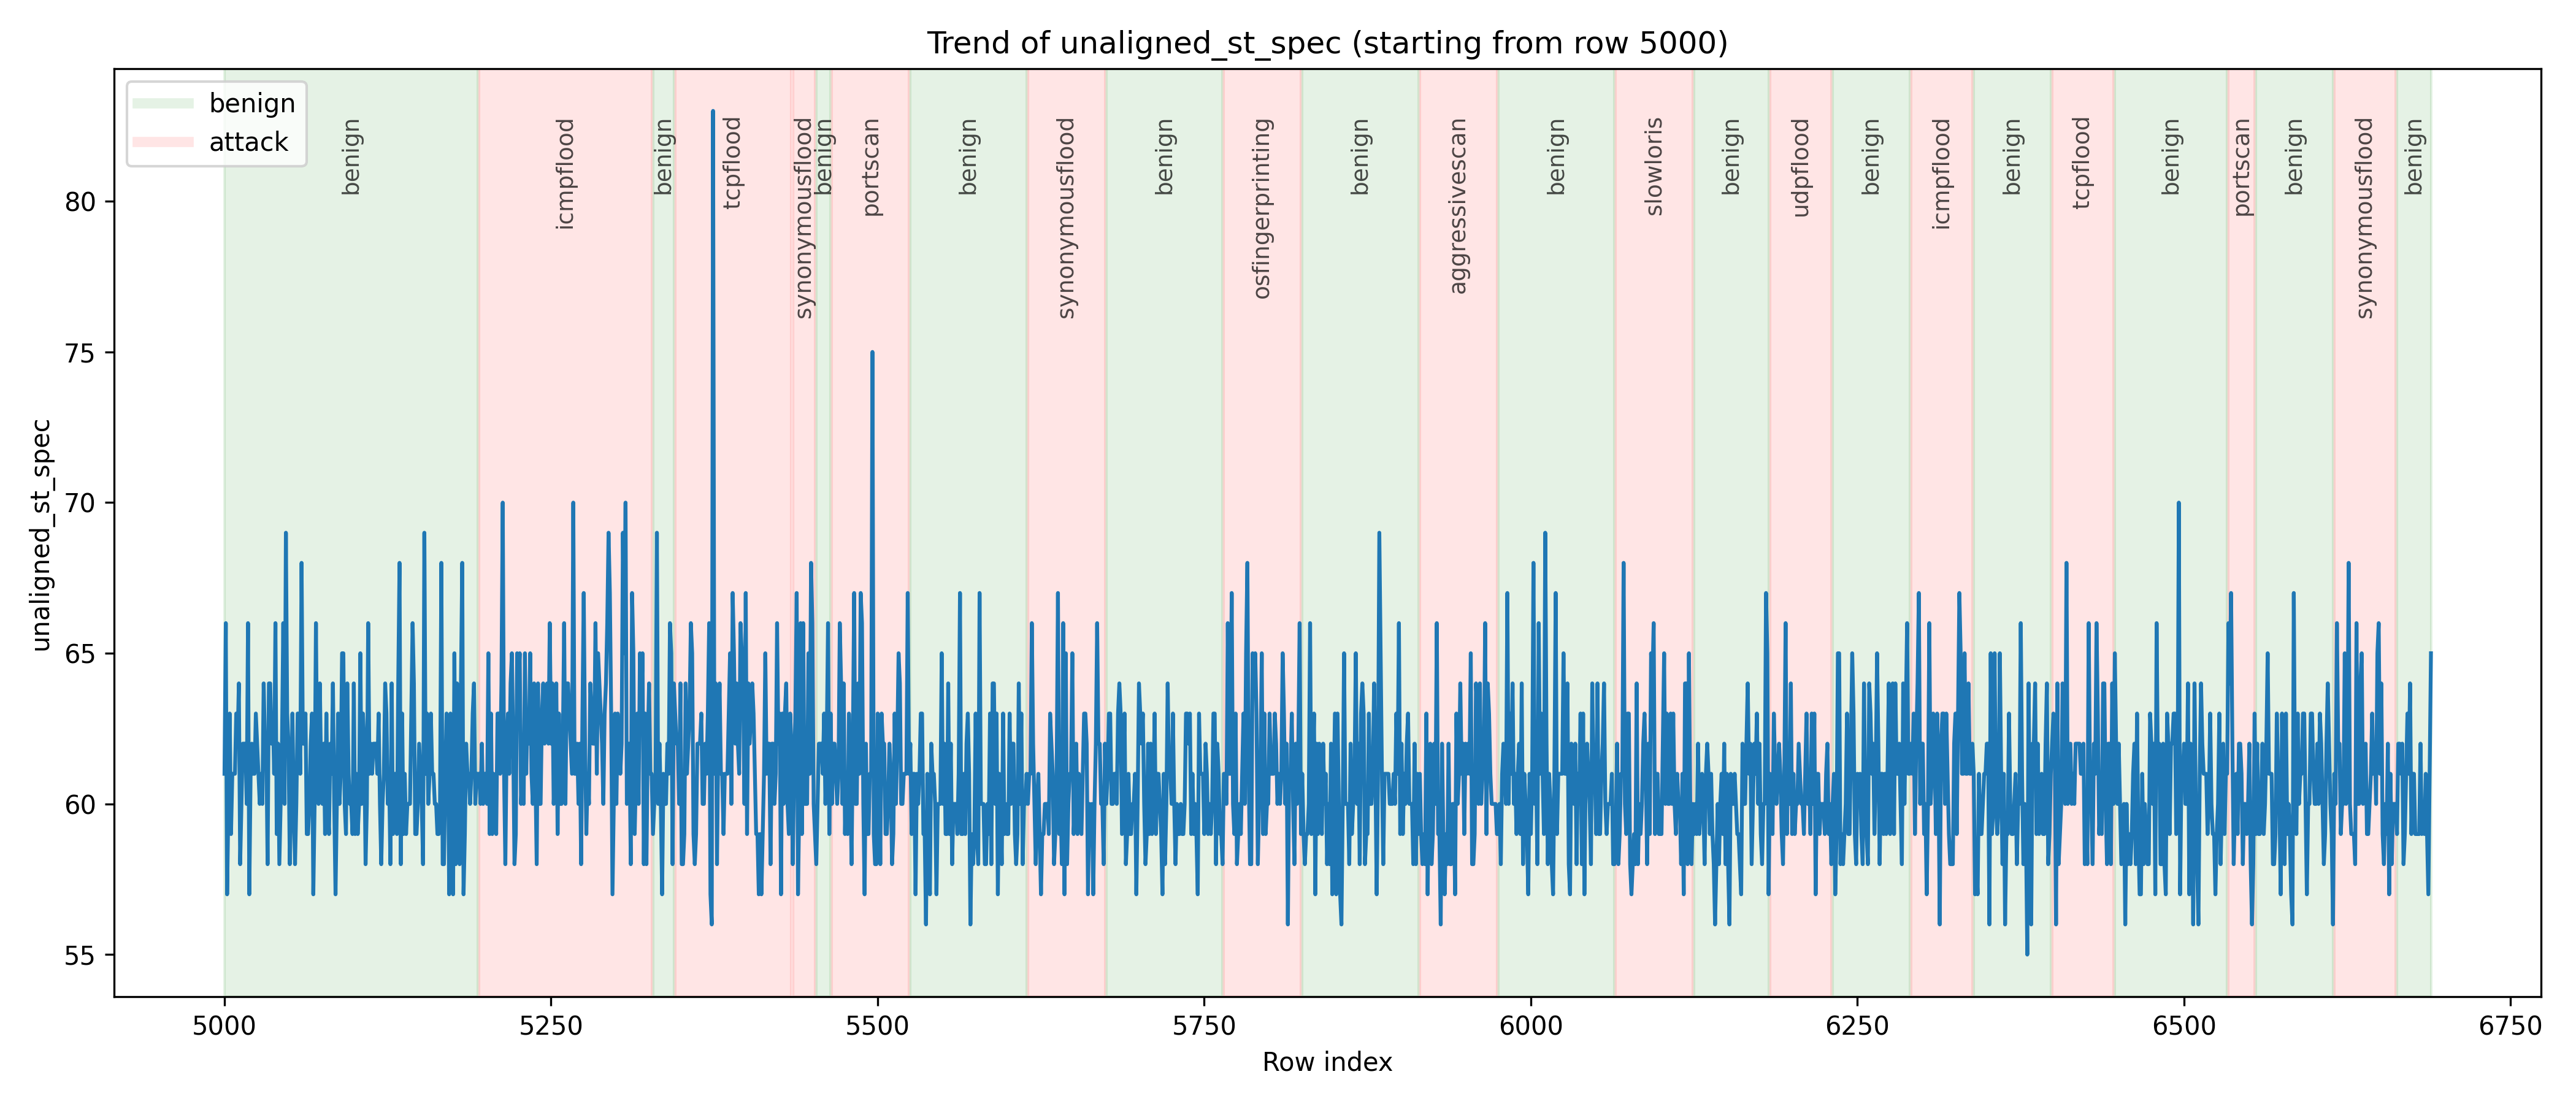
\includegraphics[width=0.9\textwidth]{pics/unaligned_st_spec.png}
    \caption{Timeline behavior of the \texttt{unaligned\_st\_spec} feature, showing little variation between benign and attack data.}
    \label{fig:unaligned_spec_timeline}
\end{figure}
\begin{figure}[H]
    \centering
    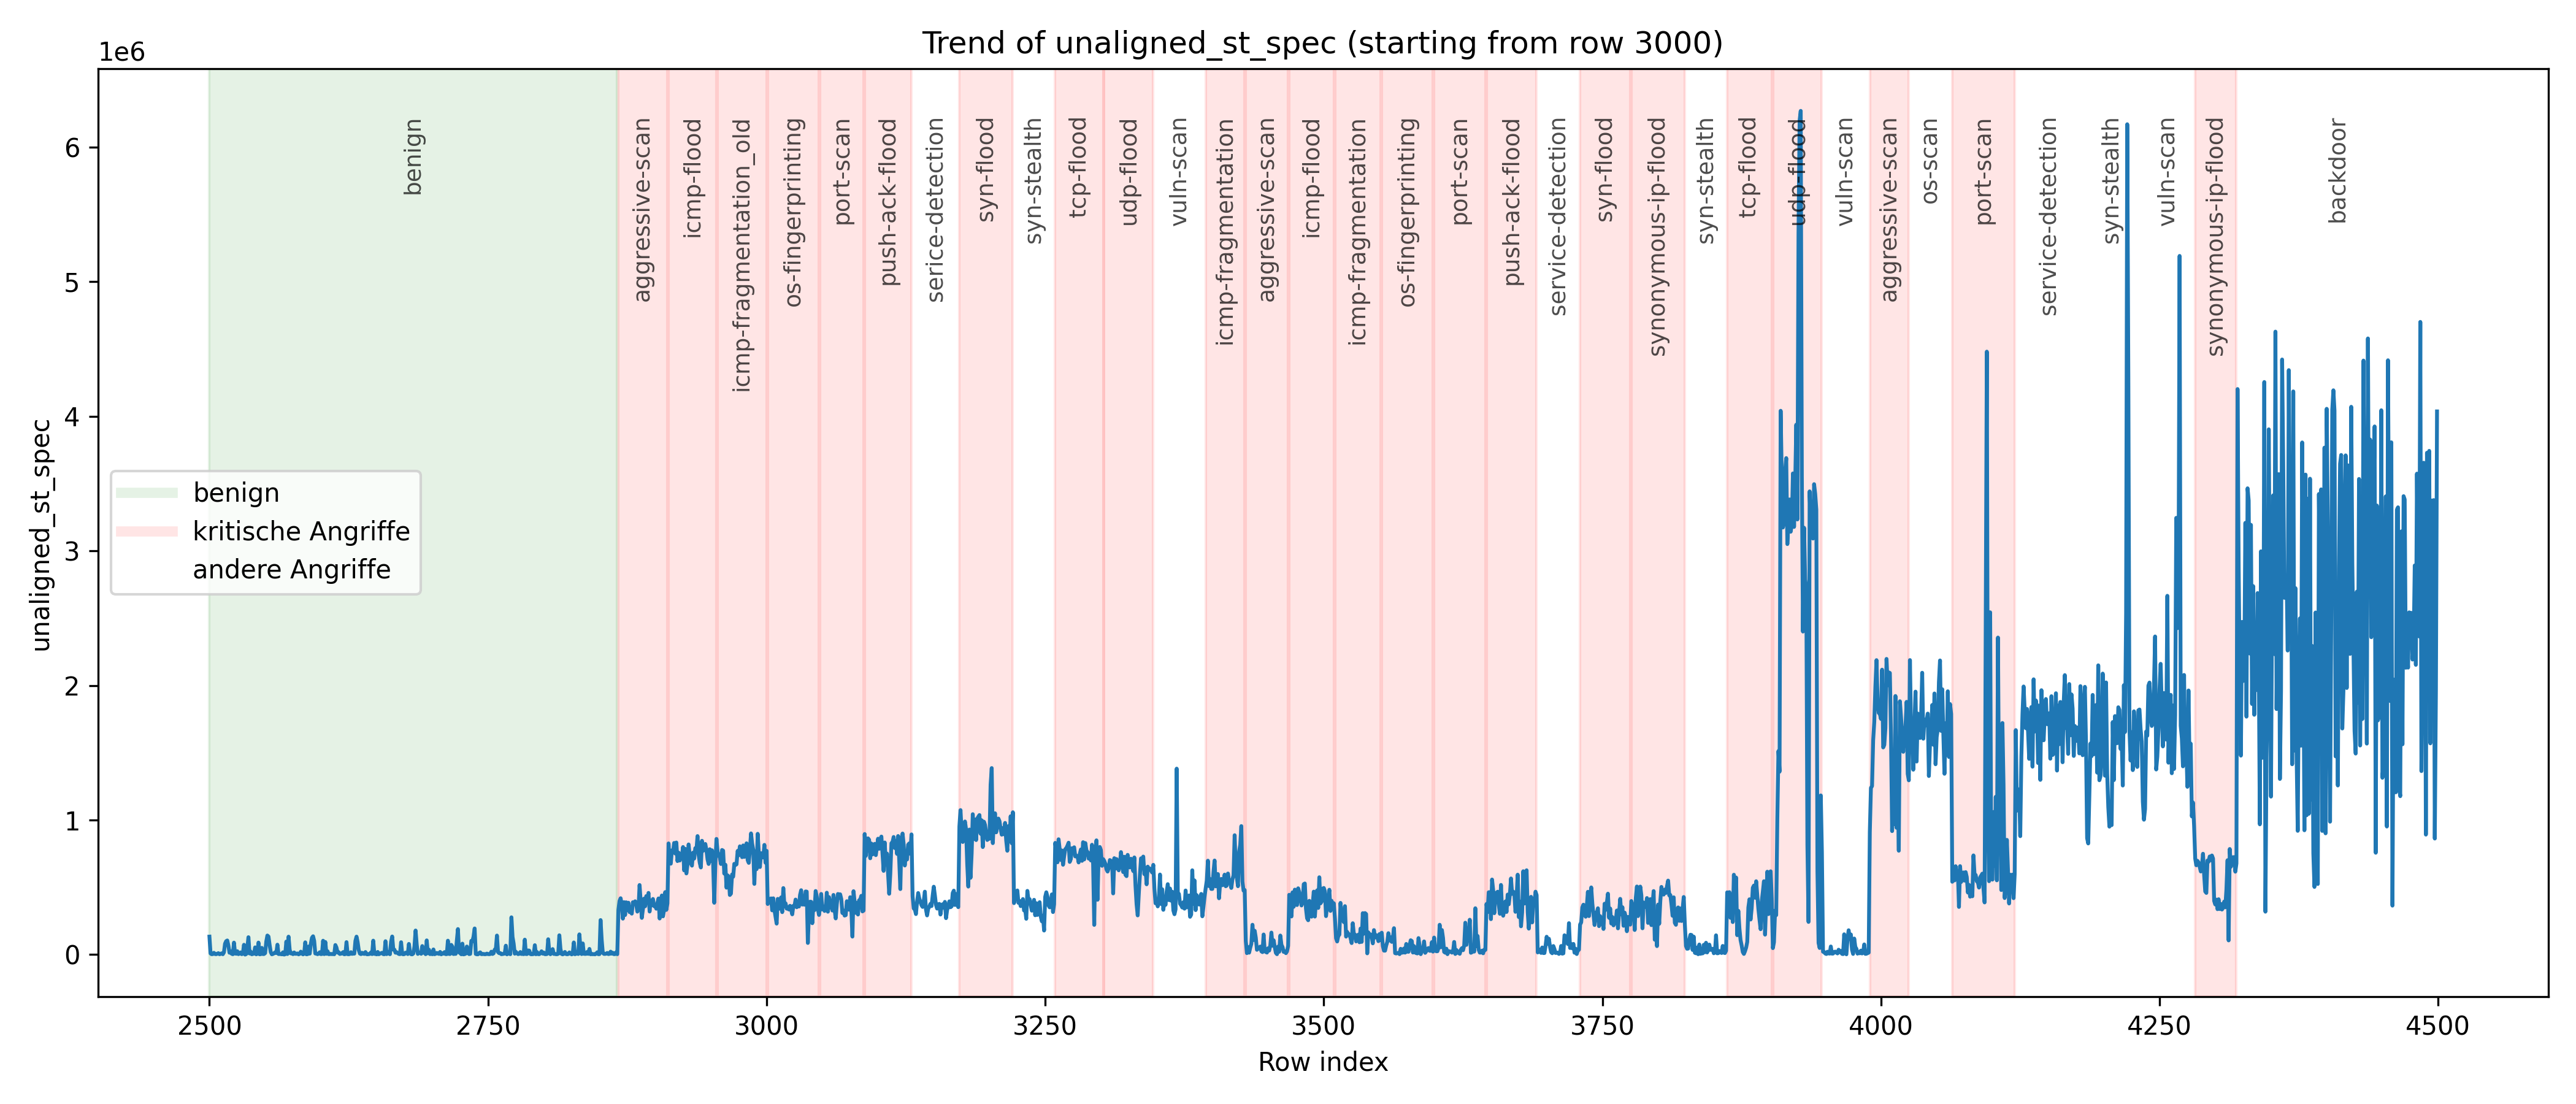
\includegraphics[width=0.9\textwidth]{pics/unaligned_st_spec_public.png}
    \caption{Timeline behavior of the \texttt{unaligned\_st\_spec} feature, from the CICEVSE2024 dataset.}
    \label{fig:unaligned_st_spec_public_timeline}
\end{figure}

